The experiement was run using the following datasets. Three configuration spaces were used which were generated from simulated robot environments, and on these environments five random sets of start and end points were generated. The three configuration spaces are presented, along with their respective points.

\begin{figure}[h]
	\centering
	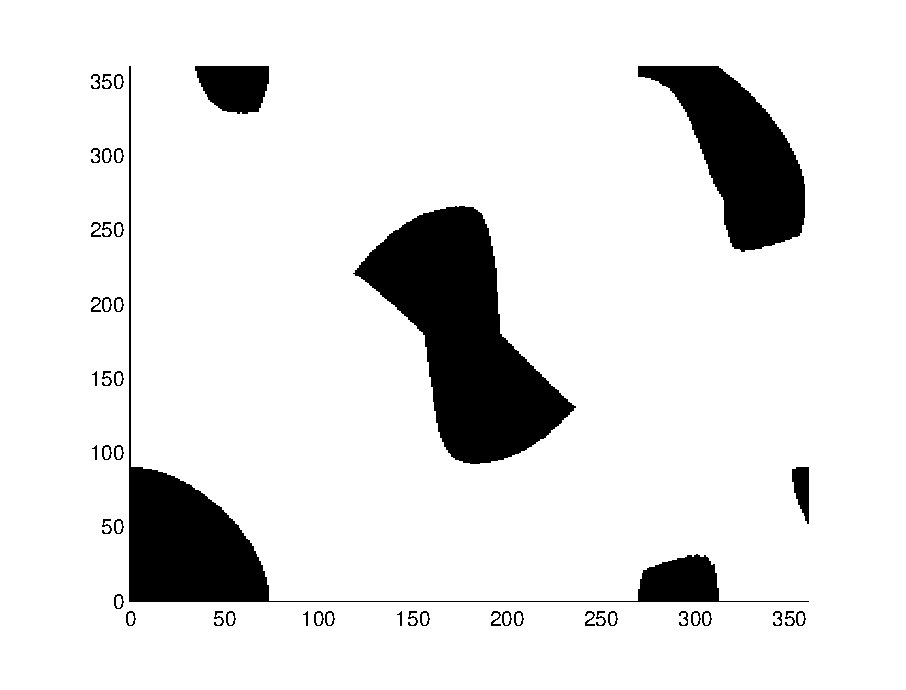
\includegraphics[width=\figWidth]{./figures/cspace2.eps}
	\caption{Configuration space \#1, the points in table \ref{tbl:pts1} were used with this space.}
	\label{fig:space1}
\end{figure}

\begin{table} [h]
\renewcommand{\arraystretch}{1.4}
	\caption{Point set \#1}
\label{tbl:pts1}
\begin{center}
		\begin{tabular}{ c | c  c  p{1.8cm} }
		X Value & Y Value \\ \hline
   7 &  104\\
   349 &  112\\
    15  & 142\\
   238   &247\\
     7   &263\\
\end{tabular}
\end{center}
\end{table}

\begin{figure}[h]
	\centering
	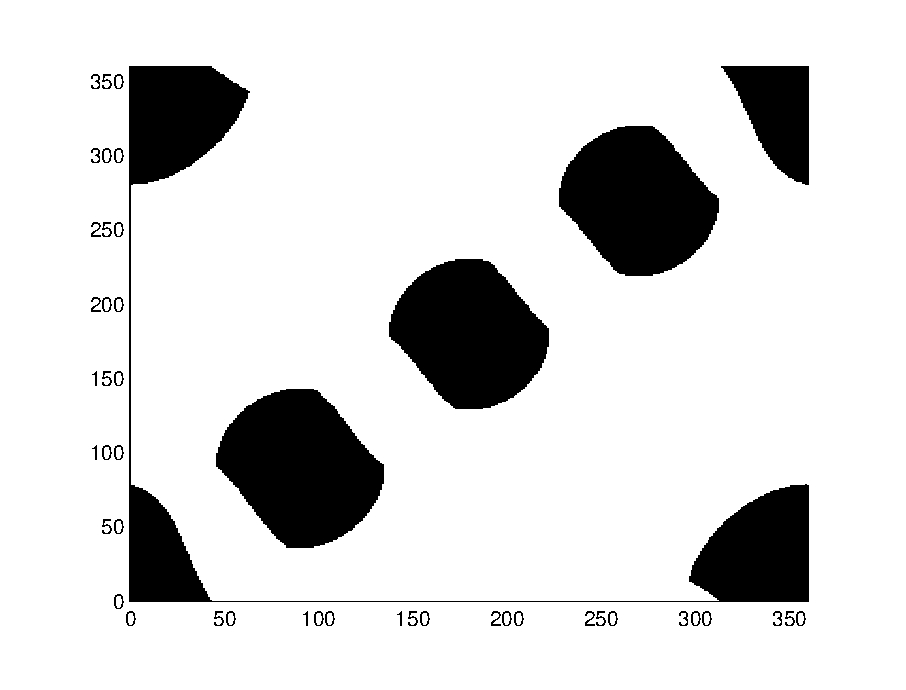
\includegraphics[width=\figWidth]{./figures/cspace3.eps}
	\caption{Configuration space \#2, the points in table \ref{tbl:pts2} were used with this space.}
	\label{fig:space2}
\end{figure}

\begin{table} [h]
\renewcommand{\arraystretch}{1.4}
	\caption{Point set \#2}
\label{tbl:pts2}
\begin{center}
		\begin{tabular}{ c | c  c  p{1.8cm} }
				X Value & Y Value \\ \hline
   311 &  159 \\
    91  & 222\\
   314   & 24\\
    58  & 219\\
   184  & 341\\
\end{tabular}
\end{center}
\end{table}

\begin{figure}[h]
	\centering
	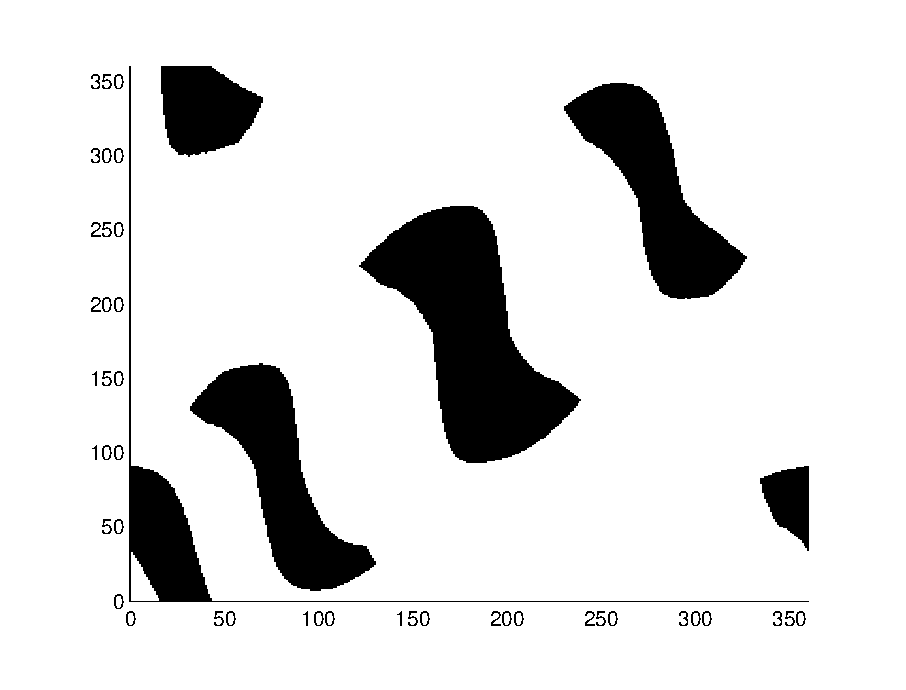
\includegraphics[width=\figWidth]{./figures/cspace4.eps}
	\caption{Configuration space \#3, the points in table \ref{tbl:pts3} were used with this space.}
	\label{fig:space3}
\end{figure}

\begin{table} [h]
\renewcommand{\arraystretch}{1.4}
	\caption{Point set \#3}
\label{tbl:pts3}
\begin{center}
		\begin{tabular}{ c | c  c  p{1.8cm} }
				X Value & Y Value \\ \hline
 155 &  318\\
   352&   146\\
   116 &  194\\
   206  & 131\\
   156   &259 \\
\end{tabular}
\end{center}
\end{table}
